\documentclass[12pt]{article}

\textwidth 16cm \textheight 23cm \evensidemargin 0cm
\oddsidemargin 0cm \topmargin -2cm
\parindent 0pt
\parskip \medskipamount


\usepackage[dutch]{babel}
\usepackage{amssymb}
\usepackage{amsmath}
\usepackage[utf8,latin1]{inputenc}
\usepackage[normalem]{ulem} % strikethrough normal text with \sout{text}
\usepackage{cancel} % strikethrough in math mode with \cancel{text}
%\usepackage{gensymb}

\usepackage{subfig}
\usepackage{graphicx}
\usepackage{graphics}
\usepackage{latexsym}
%\usepackage[latin1]{inputenc} %letters met accenten mogen in broncode gebruikt worden
\usepackage{amssymb,amsmath,amsthm} %allerlei wiskundige symbolen => http://www.ams.org/tex/amslatex.html voor read-me's
%\usepackage[small,bf,hang]{caption}
\usepackage[table]{xcolor}
\usepackage{pgf,tikz}
\usetikzlibrary{arrows}

\usepackage[pdftex]{hyperref} 
\hypersetup{setpagesize=false}
%\hypersetup{bookmarksopen}
\hypersetup{bookmarksnumbered} %voor de bookmarks in pdf de nrs zetten ook
\hypersetup{pdfborder=0.1pt} %de rand rond de links smaller maken
\hypersetup{linktocpage=true} %titels of pgnrs omkaderen in toc
\hypersetup{colorlinks=true} %kaders rond links of tekst in kleur, kaders gaan weg bij afprinten, kleur blijft


\numberwithin{equation}{section} %om de equations labels te geven die met section meegaan, dus niet gwn (1) (2) ... maar (1.1) (1.2) ...

%iets voor modulonotatie
\makeatletter
\def\imod#1{\allowbreak\mkern10mu({\operator@font mod}\,\,#1)}
\makeatother

%Getallenverzamelingen
\newcommand{\N}{\mathbb{N}}
\newcommand{\Z}{\mathbb{Z}}
\newcommand{\Q}{\mathbb{Q}}
\newcommand{\R}{\mathbb{R}}
\newcommand{\C}{\mathbb{C}}
\newcommand{\mO}{\mathcal{O}}
%<= en >= mooier maken
\renewcommand{\leq}{\leqslant}
\renewcommand{\geq}{\geqslant}

%speciale wiskunde letters: \mathcal{} of \mathfrak{}

%Nieuwe omgevingen voor definities en stellingen
\theoremstyle{plain}  \newtheorem{stel}{Stelling}[section]
\theoremstyle{plain}  \newtheorem{lemma}[stel]{Lemma}
\theoremstyle{plain}  \newtheorem{gevolg}[stel]{Gevolg}
\theoremstyle{definition}  \newtheorem{defi}[stel]{Definitie}
\theoremstyle{definition} \newtheorem{vb}[stel]{Voorbeeld}
\theoremstyle{definition} \newtheorem{vbn}[stel]{Voorbeelden}
\theoremstyle{definition}  \newtheorem{opm}[stel]{Opmerking}
\theoremstyle{plain}  \newtheorem{opdracht}{Opdracht}

\hyphenation{e-ner-zijds}
\hyphenation{ka-nons-ko-gel}
\hyphenation{schrij-ven}
\hyphenation{ka-nons-ko-gels}


\usepackage{color}
\newcommand{\todo}[1]{\textcolor{red}{\##1\#}}
\newcommand{\question}[1]{\textcolor{blue}{\##1\#}}

%\newtheorem{definitie}{Definitie}

\begin{document}

\thispagestyle{empty}

\begin{center}
 \begin{minipage}{7cm}
\begin{center}
%\aula 
%B



\includegraphics[width=5cm]{ruglogo.pdf}


 {\large
Universiteit Gent \\
Faculteit  Wetenschappen \\
Vakgroep  Wiskunde
} \end{center}\end{minipage}

\vspace{3cm}

 {\Huge\bf 
  Vullen van Vlakken en Volumes}

\baselineskip=12pt
\vspace{1.5cm}

{\large\bf  Lien Lambert }\\
\vspace{0.5cm}
{\large \bf Pieter Pareit }\\
\vspace{0.5cm}
{\large \bf Jordy Vanpoucke}\\

\baselineskip=12pt

\vspace{2cm}

 
\bigskip

{\large Academiejaar 2011-2012}

%\vspace{5cm}
%\baselineskip=1.2cm



\end{center}

\vfill

\hspace*{\fill}
\begin{minipage}{8cm}
\noindent   Project Vakdidactiek Wiskunde II
 \end{minipage}


\bigskip

\hspace*{\fill}
\begin{minipage}{8cm}
\noindent  Prof. Dr.  F. De Clerck\\
Praktijkassistent G. Maes
 \end{minipage}

\newpage
\tableofcontents 
\newpage


%\section{Vullen van Vlakken en Volumes ({\sc $V^3$})}



\section{Perfecte Vierkanten}

\subsection{Vierkant vullen met vierkanten}

Nemen we een vierkant met zijde $10$, dan kan dit vierkant gevuld worden met $100$ kleinere vierkantjes van grootte $1$. Dit is duidelijk in Figuur \ref{fig:vierkant10_1x1}. Hetzelfde vierkant kunnen we ook vullen met vierkantjes van grootte $2$, waarbij we nu $25$ kleinere vierkantjes hebben in het grote vierkant. Als we nu echter dit vierkant compleet wensen te vullen met vierkantjes van grootte $3$, dan zien we dat dit niet lukt, zie Figuur \ref{fig:vierkant10_3x3}.

\begin{figure}[ht]
  \centering
  \subfloat[in vierkantjes met zijde $1$]{\label{fig:vierkant10_1x1}\definecolor{cqcqcq}{rgb}{0.75,0.75,0.75}
\begin{tikzpicture}[scale=0.45,line cap=round,line join=round,>=triangle 45,x=1.0cm,y=1.0cm]
\draw [color=cqcqcq,dash pattern=on 2pt off 2pt, xstep=1.0cm,ystep=1.0cm] (-0.5,-0.5) grid (10.5,10.5);
\clip(-0.5,-0.5) rectangle (10.5,10.5);
\filldraw[line width=1.6pt,fill=black,fill opacity=0.1] (0,0) -- (10,0) -- (10,10) -- (0,10) -- cycle;
\filldraw[fill=black,fill opacity=0.1] (0,0) -- (1,0) -- (1,1) -- (0,1) -- cycle;
\filldraw[fill=black,fill opacity=0.1] (1,0) -- (2,0) -- (2,1) -- (1,1) -- cycle;
\filldraw[fill=black,fill opacity=0.1] (2,0) -- (3,0) -- (3,1) -- (2,1) -- cycle;
\filldraw[fill=black,fill opacity=0.1] (3,0) -- (4,0) -- (4,1) -- (3,1) -- cycle;
\filldraw[fill=black,fill opacity=0.1] (4,0) -- (5,0) -- (5,1) -- (4,1) -- cycle;
\filldraw[fill=black,fill opacity=0.1] (5,0) -- (6,0) -- (6,1) -- (5,1) -- cycle;
\filldraw[fill=black,fill opacity=0.1] (6,0) -- (7,0) -- (7,1) -- (6,1) -- cycle;
\filldraw[fill=black,fill opacity=0.1] (7,0) -- (8,0) -- (8,1) -- (7,1) -- cycle;
\filldraw[fill=black,fill opacity=0.1] (8,0) -- (9,0) -- (9,1) -- (8,1) -- cycle;
\filldraw[fill=black,fill opacity=0.1] (9,0) -- (10,0) -- (10,1) -- (9,1) -- cycle;
\filldraw[fill=black,fill opacity=0.1] (0,1) -- (1,1) -- (1,2) -- (0,2) -- cycle;
\filldraw[fill=black,fill opacity=0.1] (1,1) -- (2,1) -- (2,2) -- (1,2) -- cycle;
\filldraw[fill=black,fill opacity=0.1] (2,1) -- (3,1) -- (3,2) -- (2,2) -- cycle;
\filldraw[fill=black,fill opacity=0.1] (3,1) -- (4,1) -- (4,2) -- (3,2) -- cycle;
\filldraw[fill=black,fill opacity=0.1] (4,1) -- (5,1) -- (5,2) -- (4,2) -- cycle;
\filldraw[fill=black,fill opacity=0.1] (5,1) -- (6,1) -- (6,2) -- (5,2) -- cycle;
\filldraw[fill=black,fill opacity=0.1] (6,1) -- (7,1) -- (7,2) -- (6,2) -- cycle;
\filldraw[fill=black,fill opacity=0.1] (7,1) -- (8,1) -- (8,2) -- (7,2) -- cycle;
\filldraw[fill=black,fill opacity=0.1] (8,1) -- (9,1) -- (9,2) -- (8,2) -- cycle;
\filldraw[fill=black,fill opacity=0.1] (9,1) -- (10,1) -- (10,2) -- (9,2) -- cycle;
\filldraw[fill=black,fill opacity=0.1] (0,2) -- (1,2) -- (1,3) -- (0,3) -- cycle;
\filldraw[fill=black,fill opacity=0.1] (1,2) -- (2,2) -- (2,3) -- (1,3) -- cycle;
\filldraw[fill=black,fill opacity=0.1] (2,2) -- (3,2) -- (3,3) -- (2,3) -- cycle;
\filldraw[fill=black,fill opacity=0.1] (3,2) -- (4,2) -- (4,3) -- (3,3) -- cycle;
\filldraw[fill=black,fill opacity=0.1] (4,2) -- (5,2) -- (5,3) -- (4,3) -- cycle;
\filldraw[fill=black,fill opacity=0.1] (5,2) -- (6,2) -- (6,3) -- (5,3) -- cycle;
\filldraw[fill=black,fill opacity=0.1] (6,2) -- (7,2) -- (7,3) -- (6,3) -- cycle;
\filldraw[fill=black,fill opacity=0.1] (7,2) -- (8,2) -- (8,3) -- (7,3) -- cycle;
\filldraw[fill=black,fill opacity=0.1] (8,2) -- (9,2) -- (9,3) -- (8,3) -- cycle;
\filldraw[fill=black,fill opacity=0.1] (9,2) -- (10,2) -- (10,3) -- (9,3) -- cycle;
\filldraw[fill=black,fill opacity=0.1] (0,3) -- (1,3) -- (1,4) -- (0,4) -- cycle;
\filldraw[fill=black,fill opacity=0.1] (1,3) -- (2,3) -- (2,4) -- (1,4) -- cycle;
\filldraw[fill=black,fill opacity=0.1] (2,3) -- (3,3) -- (3,4) -- (2,4) -- cycle;
\filldraw[fill=black,fill opacity=0.1] (3,3) -- (4,3) -- (4,4) -- (3,4) -- cycle;
\filldraw[fill=black,fill opacity=0.1] (4,3) -- (5,3) -- (5,4) -- (4,4) -- cycle;
\filldraw[fill=black,fill opacity=0.1] (5,3) -- (6,3) -- (6,4) -- (5,4) -- cycle;
\filldraw[fill=black,fill opacity=0.1] (6,3) -- (7,3) -- (7,4) -- (6,4) -- cycle;
\filldraw[fill=black,fill opacity=0.1] (7,3) -- (8,3) -- (8,4) -- (7,4) -- cycle;
\filldraw[fill=black,fill opacity=0.1] (8,3) -- (9,3) -- (9,4) -- (8,4) -- cycle;
\filldraw[fill=black,fill opacity=0.1] (9,3) -- (10,3) -- (10,4) -- (9,4) -- cycle;
\filldraw[fill=black,fill opacity=0.1] (0,4) -- (1,4) -- (1,5) -- (0,5) -- cycle;
\filldraw[fill=black,fill opacity=0.1] (1,4) -- (2,4) -- (2,5) -- (1,5) -- cycle;
\filldraw[fill=black,fill opacity=0.1] (2,4) -- (3,4) -- (3,5) -- (2,5) -- cycle;
\filldraw[fill=black,fill opacity=0.1] (3,4) -- (4,4) -- (4,5) -- (3,5) -- cycle;
\filldraw[fill=black,fill opacity=0.1] (4,4) -- (5,4) -- (5,5) -- (4,5) -- cycle;
\filldraw[fill=black,fill opacity=0.1] (5,4) -- (6,4) -- (6,5) -- (5,5) -- cycle;
\filldraw[fill=black,fill opacity=0.1] (6,4) -- (7,4) -- (7,5) -- (6,5) -- cycle;
\filldraw[fill=black,fill opacity=0.1] (7,4) -- (8,4) -- (8,5) -- (7,5) -- cycle;
\filldraw[fill=black,fill opacity=0.1] (8,4) -- (9,4) -- (9,5) -- (8,5) -- cycle;
\filldraw[fill=black,fill opacity=0.1] (9,4) -- (10,4) -- (10,5) -- (9,5) -- cycle;
\filldraw[fill=black,fill opacity=0.1] (0,5) -- (1,5) -- (1,6) -- (0,6) -- cycle;
\filldraw[fill=black,fill opacity=0.1] (1,5) -- (2,5) -- (2,6) -- (1,6) -- cycle;
\filldraw[fill=black,fill opacity=0.1] (2,5) -- (3,5) -- (3,6) -- (2,6) -- cycle;
\filldraw[fill=black,fill opacity=0.1] (3,5) -- (4,5) -- (4,6) -- (3,6) -- cycle;
\filldraw[fill=black,fill opacity=0.1] (4,5) -- (5,5) -- (5,6) -- (4,6) -- cycle;
\filldraw[fill=black,fill opacity=0.1] (5,5) -- (6,5) -- (6,6) -- (5,6) -- cycle;
\filldraw[fill=black,fill opacity=0.1] (6,5) -- (7,5) -- (7,6) -- (6,6) -- cycle;
\filldraw[fill=black,fill opacity=0.1] (7,5) -- (8,5) -- (8,6) -- (7,6) -- cycle;
\filldraw[fill=black,fill opacity=0.1] (8,5) -- (9,5) -- (9,6) -- (8,6) -- cycle;
\filldraw[fill=black,fill opacity=0.1] (9,5) -- (10,5) -- (10,6) -- (9,6) -- cycle;
\filldraw[fill=black,fill opacity=0.1] (0,6) -- (1,6) -- (1,7) -- (0,7) -- cycle;
\filldraw[fill=black,fill opacity=0.1] (1,6) -- (2,6) -- (2,7) -- (1,7) -- cycle;
\filldraw[fill=black,fill opacity=0.1] (2,6) -- (3,6) -- (3,7) -- (2,7) -- cycle;
\filldraw[fill=black,fill opacity=0.1] (3,6) -- (4,6) -- (4,7) -- (3,7) -- cycle;
\filldraw[fill=black,fill opacity=0.1] (4,6) -- (5,6) -- (5,7) -- (4,7) -- cycle;
\filldraw[fill=black,fill opacity=0.1] (5,6) -- (6,6) -- (6,7) -- (5,7) -- cycle;
\filldraw[fill=black,fill opacity=0.1] (6,6) -- (7,6) -- (7,7) -- (6,7) -- cycle;
\filldraw[fill=black,fill opacity=0.1] (7,6) -- (8,6) -- (8,7) -- (7,7) -- cycle;
\filldraw[fill=black,fill opacity=0.1] (8,6) -- (9,6) -- (9,7) -- (8,7) -- cycle;
\filldraw[fill=black,fill opacity=0.1] (9,6) -- (10,6) -- (10,7) -- (9,7) -- cycle;
\filldraw[fill=black,fill opacity=0.1] (0,7) -- (1,7) -- (1,8) -- (0,8) -- cycle;
\filldraw[fill=black,fill opacity=0.1] (1,7) -- (2,7) -- (2,8) -- (1,8) -- cycle;
\filldraw[fill=black,fill opacity=0.1] (2,7) -- (3,7) -- (3,8) -- (2,8) -- cycle;
\filldraw[fill=black,fill opacity=0.1] (3,7) -- (4,7) -- (4,8) -- (3,8) -- cycle;
\filldraw[fill=black,fill opacity=0.1] (4,7) -- (5,7) -- (5,8) -- (4,8) -- cycle;
\filldraw[fill=black,fill opacity=0.1] (5,7) -- (6,7) -- (6,8) -- (5,8) -- cycle;
\filldraw[fill=black,fill opacity=0.1] (6,7) -- (7,7) -- (7,8) -- (6,8) -- cycle;
\filldraw[fill=black,fill opacity=0.1] (7,7) -- (8,7) -- (8,8) -- (7,8) -- cycle;
\filldraw[fill=black,fill opacity=0.1] (8,7) -- (9,7) -- (9,8) -- (8,8) -- cycle;
\filldraw[fill=black,fill opacity=0.1] (9,7) -- (10,7) -- (10,8) -- (9,8) -- cycle;
\filldraw[fill=black,fill opacity=0.1] (0,8) -- (1,8) -- (1,9) -- (0,9) -- cycle;
\filldraw[fill=black,fill opacity=0.1] (1,8) -- (2,8) -- (2,9) -- (1,9) -- cycle;
\filldraw[fill=black,fill opacity=0.1] (2,8) -- (3,8) -- (3,9) -- (2,9) -- cycle;
\filldraw[fill=black,fill opacity=0.1] (3,8) -- (4,8) -- (4,9) -- (3,9) -- cycle;
\filldraw[fill=black,fill opacity=0.1] (4,8) -- (5,8) -- (5,9) -- (4,9) -- cycle;
\filldraw[fill=black,fill opacity=0.1] (5,8) -- (6,8) -- (6,9) -- (5,9) -- cycle;
\filldraw[fill=black,fill opacity=0.1] (6,8) -- (7,8) -- (7,9) -- (6,9) -- cycle;
\filldraw[fill=black,fill opacity=0.1] (7,8) -- (8,8) -- (8,9) -- (7,9) -- cycle;
\filldraw[fill=black,fill opacity=0.1] (8,8) -- (9,8) -- (9,9) -- (8,9) -- cycle;
\filldraw[fill=black,fill opacity=0.1] (9,8) -- (10,8) -- (10,9) -- (9,9) -- cycle;
\filldraw[fill=black,fill opacity=0.1] (0,9) -- (1,9) -- (1,10) -- (0,10) -- cycle;
\filldraw[fill=black,fill opacity=0.1] (1,9) -- (2,9) -- (2,10) -- (1,10) -- cycle;
\filldraw[fill=black,fill opacity=0.1] (2,9) -- (3,9) -- (3,10) -- (2,10) -- cycle;
\filldraw[fill=black,fill opacity=0.1] (3,9) -- (4,9) -- (4,10) -- (3,10) -- cycle;
\filldraw[fill=black,fill opacity=0.1] (4,9) -- (5,9) -- (5,10) -- (4,10) -- cycle;
\filldraw[fill=black,fill opacity=0.1] (5,9) -- (6,9) -- (6,10) -- (5,10) -- cycle;
\filldraw[fill=black,fill opacity=0.1] (6,9) -- (7,9) -- (7,10) -- (6,10) -- cycle;
\filldraw[fill=black,fill opacity=0.1] (7,9) -- (8,9) -- (8,10) -- (7,10) -- cycle;
\filldraw[fill=black,fill opacity=0.1] (8,9) -- (9,9) -- (9,10) -- (8,10) -- cycle;
\filldraw[fill=black,fill opacity=0.1] (9,9) -- (10,9) -- (10,10) -- (9,10) -- cycle;
\end{tikzpicture}
}
  \subfloat[in vierkantjes met zijde $2$]{\label{fig:vierkant10_2x2}\definecolor{cqcqcq}{rgb}{0.75,0.75,0.75}
\begin{tikzpicture}[scale=0.45,line cap=round,line join=round,>=triangle 45,x=1.0cm,y=1.0cm]
\draw [color=cqcqcq,dash pattern=on 2pt off 2pt, xstep=1.0cm,ystep=1.0cm] (-0.5,-0.5) grid (10.5,10.5);
\clip(-0.5,-0.5) rectangle (10.5,10.5);
\filldraw[line width=1.6pt,fill=black,fill opacity=0.1] (0,0) -- (10,0) -- (10,10) -- (0,10) -- cycle;
\filldraw[fill=black,fill opacity=0.1] (0,0) -- (2,0) -- (2,2) -- (0,2) -- cycle;
\filldraw[fill=black,fill opacity=0.1] (2,0) -- (4,0) -- (4,2) -- (2,2) -- cycle;
\filldraw[fill=black,fill opacity=0.1] (4,0) -- (6,0) -- (6,2) -- (4,2) -- cycle;
\filldraw[fill=black,fill opacity=0.1] (6,0) -- (8,0) -- (8,2) -- (6,2) -- cycle;
\filldraw[fill=black,fill opacity=0.1] (8,0) -- (10,0) -- (10,2) -- (8,2) -- cycle;
\filldraw[fill=black,fill opacity=0.1] (0,2) -- (2,2) -- (2,4) -- (0,4) -- cycle;
\filldraw[fill=black,fill opacity=0.1] (2,2) -- (4,2) -- (4,4) -- (2,4) -- cycle;
\filldraw[fill=black,fill opacity=0.1] (4,2) -- (6,2) -- (6,4) -- (4,4) -- cycle;
\filldraw[fill=black,fill opacity=0.1] (6,2) -- (8,2) -- (8,4) -- (6,4) -- cycle;
\filldraw[fill=black,fill opacity=0.1] (8,2) -- (10,2) -- (10,4) -- (8,4) -- cycle;
\filldraw[fill=black,fill opacity=0.1] (0,4) -- (2,4) -- (2,6) -- (0,6) -- cycle;
\filldraw[fill=black,fill opacity=0.1] (2,4) -- (4,4) -- (4,6) -- (2,6) -- cycle;
\filldraw[fill=black,fill opacity=0.1] (4,4) -- (6,4) -- (6,6) -- (4,6) -- cycle;
\filldraw[fill=black,fill opacity=0.1] (6,4) -- (8,4) -- (8,6) -- (6,6) -- cycle;
\filldraw[fill=black,fill opacity=0.1] (8,4) -- (10,4) -- (10,6) -- (8,6) -- cycle;
\filldraw[fill=black,fill opacity=0.1] (0,6) -- (2,6) -- (2,8) -- (0,8) -- cycle;
\filldraw[fill=black,fill opacity=0.1] (2,6) -- (4,6) -- (4,8) -- (2,8) -- cycle;
\filldraw[fill=black,fill opacity=0.1] (4,6) -- (6,6) -- (6,8) -- (4,8) -- cycle;
\filldraw[fill=black,fill opacity=0.1] (6,6) -- (8,6) -- (8,8) -- (6,8) -- cycle;
\filldraw[fill=black,fill opacity=0.1] (8,6) -- (10,6) -- (10,8) -- (8,8) -- cycle;
\filldraw[fill=black,fill opacity=0.1] (0,8) -- (2,8) -- (2,10) -- (0,10) -- cycle;
\filldraw[fill=black,fill opacity=0.1] (2,8) -- (4,8) -- (4,10) -- (2,10) -- cycle;
\filldraw[fill=black,fill opacity=0.1] (4,8) -- (6,8) -- (6,10) -- (4,10) -- cycle;
\filldraw[fill=black,fill opacity=0.1] (6,8) -- (8,8) -- (8,10) -- (6,10) -- cycle;
\filldraw[fill=black,fill opacity=0.1] (8,8) -- (10,8) -- (10,10) -- (8,10) -- cycle;
\end{tikzpicture}
}
  \subfloat[in vierkantjes met zijde $3$]{\label{fig:vierkant10_3x3}\definecolor{cqcqcq}{rgb}{0.75,0.75,0.75}
\begin{tikzpicture}[scale=0.4,line cap=round,line join=round,>=triangle 45,x=1.0cm,y=1.0cm]
\draw [color=cqcqcq,dash pattern=on 2pt off 2pt, xstep=1.0cm,ystep=1.0cm] (-0.5,-0.5) grid (10.5,10.5);
\clip(-0.5,-0.5) rectangle (10.5,10.5);
\filldraw[line width=1.6pt,fill=black,fill opacity=0.1] (0,0) -- (10,0) -- (10,10) -- (0,10) -- cycle;
\filldraw[fill=black,fill opacity=0.1] (0,0) -- (3,0) -- (3,3) -- (0,3) -- cycle;
\filldraw[fill=black,fill opacity=0.1] (3,0) -- (6,0) -- (6,3) -- (3,3) -- cycle;
\filldraw[fill=black,fill opacity=0.1] (6,0) -- (9,0) -- (9,3) -- (6,3) -- cycle;
\filldraw[fill=black,fill opacity=0.1] (0,3) -- (3,3) -- (3,6) -- (0,6) -- cycle;
\filldraw[fill=black,fill opacity=0.1] (3,3) -- (6,3) -- (6,6) -- (3,6) -- cycle;
\filldraw[fill=black,fill opacity=0.1] (6,3) -- (9,3) -- (9,6) -- (6,6) -- cycle;
\filldraw[fill=black,fill opacity=0.1] (0,6) -- (3,6) -- (3,9) -- (0,9) -- cycle;
\filldraw[fill=black,fill opacity=0.1] (3,6) -- (6,6) -- (6,9) -- (3,9) -- cycle;
\filldraw[fill=black,fill opacity=0.1] (6,6) -- (9,6) -- (9,9) -- (6,9) -- cycle;
\end{tikzpicture}
}
  \caption{Verdelen van een vierkant met zijde $10$.}
  \label{fig:vierkant10}
\end{figure}

We kunnen het vierkant met zijde $10$ vullen met $9$ vierkanten van zijde $3$. Er blijven $19$ kleinere vierkantjes van zijde $1$ over. We kunnen dit ook als volgt zien: als we de zijde van grootte $10$ delen door de grootte van de kleinere zijde $3$, dan is de rest $1$ en het quotiënt $3$. We hebben dus
$$
10 = 3\cdot 3 + 1.
$$
Het gaat uiteraard over vierkanten. Dus om met de oppervlakten te werken moeten we links en rechts kwadrateren, we krijgen dus
\begin{align*}
  10^2  &= (3\cdot 3 + 1)^2\\
  \Leftrightarrow 100   &= (3\cdot 3)^2 + 2\cdot 3\cdot 3\cdot 1 + 1^2\\
  \Leftrightarrow 100   &= 81 + 19
\end{align*}

In het linkerlid staat dus de oppervlakte van het groter vierkant. Het rechter lid is opgesplitst in het totale oppervlakte van de kleinere vierkanten plus wat er nog overblijft als rest.

Vul nu zelf de vierkanten met zijde $9$ uit Figuur \ref{fig:vierkant9}. Eerst met kleinere vierkantjes van grootte $1$, dan met kleinere vierkantjes van grootte $2$ en uiteindelijk met kleinere vierkantjes van grootte $3$. Gebruik wat je kent over delen van getallen en rest bij deling om het resultaat te verklaren.

\begin{figure}[ht]
  \centering
  \subfloat[in vierkantjes met zijde $1$]{\definecolor{cqcqcq}{rgb}{0.75,0.75,0.75}
\begin{tikzpicture}[scale=0.45,line cap=round,line join=round,>=triangle 45,x=1.0cm,y=1.0cm]
\draw [color=cqcqcq,dash pattern=on 2pt off 2pt, xstep=1.0cm,ystep=1.0cm] (-0.5,-0.5) grid (9.5,9.5);
\clip(-0.5,-0.5) rectangle (9.5,9.5);
\filldraw[line width=1.6pt,fill=black,fill opacity=0.1] (0,0) -- (9,0) -- (9,9) -- (0,9) -- cycle;
\end{tikzpicture}
}
  \subfloat[in vierkantjes met zijde $2$]{\definecolor{cqcqcq}{rgb}{0.75,0.75,0.75}
\begin{tikzpicture}[scale=0.45,line cap=round,line join=round,>=triangle 45,x=1.0cm,y=1.0cm]
\draw [color=cqcqcq,dash pattern=on 2pt off 2pt, xstep=1.0cm,ystep=1.0cm] (-0.5,-0.5) grid (9.5,9.5);
\clip(-0.5,-0.5) rectangle (9.5,9.5);
\filldraw[line width=1.6pt,fill=black,fill opacity=0.1] (0,0) -- (9,0) -- (9,9) -- (0,9) -- cycle;
\end{tikzpicture}
}
  \subfloat[in vierkantjes met zijde $3$]{\definecolor{cqcqcq}{rgb}{0.75,0.75,0.75}
\begin{tikzpicture}[scale=0.45,line cap=round,line join=round,>=triangle 45,x=1.0cm,y=1.0cm]
\draw [color=cqcqcq,dash pattern=on 2pt off 2pt, xstep=1.0cm,ystep=1.0cm] (-0.5,-0.5) grid (9.5,9.5);
\clip(-0.5,-0.5) rectangle (9.5,9.5);
\filldraw[line width=1.6pt,fill=black,fill opacity=0.1] (0,0) -- (9,0) -- (9,9) -- (0,9) -- cycle;
\end{tikzpicture}
}
  \caption{Verdelen van een vierkant met zijde $9$.}
  \label{fig:vierkant9}
\end{figure}

Verklaring:
\answer[4cm]{Elk vierkant waarvan de zijden een natuurlijke (dus geen komma getallen) grootte hebben volledig opgevuld worden met kleinere vierkantjes van grootte $1$. Omdat $9$ niet deelbaar is door $2$ blijven we met een rest zitten. We kunnen deze rest als volgt berekenen: de rest bij deling van $9$ door $2$ is $1$ en het quotiënt is $4$,  we hebben dus $9=4\cdot 2 + 1$, dit links en rechts kwadrateren geeft $9^2=(4\cdot 2 + 1)^2\Leftrightarrow 9^2=(4\cdot 2)^2 + 2\cdot 4\cdot 2 + 1^2 \Leftrightarrow 81 = 64 + 16 + 1 \Leftrightarrow 81 = 64 + 17$. Het vierkant van zijde $9$ vullen met vierkanten van zijde $3$ lukt volledig omdat $3$ een deler is van $9$.}

We kunnen dit gaan veralgemenen voor een groot vierkant met zijde $a$ en kleinere vierkanten met zijde $d$. Er zal dus steeds gelden
$$
a = q\cdot d + r
$$
waarbij $q$ het aantal keer is dat we $d$ in $a$ krijgen en $r$ de rest is die dan nog overblijft. Als we dit dan links en rechts kwadrateren, dan krijgen we
\begin{align*}
  a^2  &= (q\cdot d + r)^2\\
  \Leftrightarrow a^2   &= (q\cdot d)^2 + 2\cdot q\cdot d\cdot r + r^2\;.\\
\end{align*}
In een groot vierkant zal de oppervlakte dus $a^2$ zijn en het wordt gevuld met $q^2$ kleinere vierkanten van oppervlakte $d^2$. In het totaal blijft een oppervlakte van $2\cdot q\cdot r + r^2$ over. Laten we deze restoppervlakte nu de overschot noemen. Dit kunnen we ontleden in een stukje oppervlakte van $q\cdot r$ dat rechts overblijft, een stukje oppervlakte van $q\cdot r$ dat bovenaan overblijft en een stukje oppervlakte $r^2$ dat rechtsboven overblijft.

Duid deze nog aan op Figuur \ref{fig:vierkant10_4x4} waarbij een groot vierkant met zijde $10$ werd opgedeeld in vierkanten met zijde $4$.
\answer{Het blauwe en rode stukje hebben oppervlakte $q\cdot r$, het groene stukje heeft oppervlakte $r^2$.}

\begin{figure}[ht]
  \centering
  \definecolor{zzccqq}{rgb}{0.6,0.8,0}
\definecolor{wwwwff}{rgb}{0.4,0.4,1}
\definecolor{ffwwtt}{rgb}{1,0.4,0.2}
\definecolor{cqcqcq}{rgb}{0.75,0.75,0.75}
\begin{tikzpicture}[scale=0.6,line cap=round,line join=round,>=triangle 45,x=1.0cm,y=1.0cm]
\draw [color=cqcqcq,dash pattern=on 1pt off 1pt, xstep=1.0cm,ystep=1.0cm] (-0.5,-0.5) grid (10.5,10.5);
\clip(-0.5,-0.5) rectangle (10.5,10.5);
\filldraw[fill=black,fill opacity=0.1] (0,0) -- (10,0) -- (10,10) -- (0,10) -- cycle;
\filldraw[fill=black,fill opacity=0.1] (0,0) -- (4,0) -- (4,4) -- (0,4) -- cycle;
\filldraw[fill=black,fill opacity=0.1] (4,0) -- (8,0) -- (8,4) -- (4,4) -- cycle;
\filldraw[fill=black,fill opacity=0.1] (0,4) -- (4,4) -- (4,8) -- (0,8) -- cycle;
\filldraw[fill=black,fill opacity=0.1] (4,4) -- (8,4) -- (8,8) -- (4,8) -- cycle;
\filldraw[color=ffwwtt,fill=ffwwtt,fill opacity=0.1] (8,0) -- (10,0) -- (10,8) -- (8,8) -- cycle;
\filldraw[color=wwwwff,fill=wwwwff,fill opacity=0.1] (0,10) -- (0,8) -- (8,8) -- (8,10) -- cycle;
\filldraw[color=zzccqq,fill=zzccqq,fill opacity=0.1] (8,8) -- (10,8) -- (10,10) -- (8,10) -- cycle;
\filldraw [color=ffwwtt] (8,0)-- (10,0);
\draw [color=ffwwtt] (10,0)-- (10,8);
\draw [color=ffwwtt] (10,8)-- (8,8);
\draw [color=ffwwtt] (8,8)-- (8,0);
\draw [color=wwwwff] (0,10)-- (0,8);
\draw [color=wwwwff] (0,8)-- (8,8);
\draw [color=wwwwff] (8,8)-- (8,10);
\draw [color=wwwwff] (8,10)-- (0,10);
\draw [color=zzccqq] (8,8)-- (10,8);
\draw [color=zzccqq] (10,8)-- (10,10);
\draw [color=zzccqq] (10,10)-- (8,10);
\draw [color=zzccqq] (8,10)-- (8,8);
\end{tikzpicture}

  \caption{Rest van een vierkant van grootte 10 verdeeld in vierkantjes van grootte 4.}
  \label{fig:vierkant10_4x4}
\end{figure}

\newpage
\subsection{Perfecte vierkanten}

Het probleem om een vierkant te vullen met kleinere vierkanten wordt heel wat uitdagender en een gans stuk moeilijker als we eisen dat alle vierkanten een andere grootte moeten hebben. Indien een vierkant volledig gevuld wordt met kleinere vierkanten die allemaal een andere grootte hebben, dan spreken we van een {\bf perfect vierkant}. Het aantal kleinere vierkanten dat het grootte vierkant bevat wordt de {\bf orde} van het perfecte vierkant genoemd. Het vierkant met de kleinste orde staat in Figuur \ref{fig:pv21}.

\begin{figure}[ht]
  \centering
  {\small
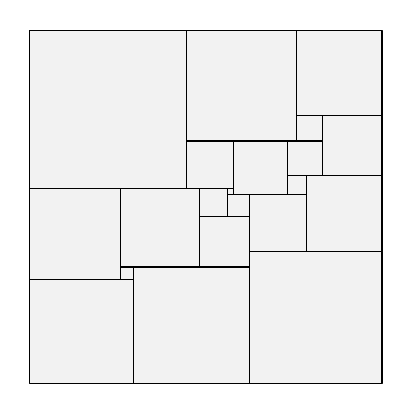
\begin{tikzpicture}[scale=0.04,line cap=round,line join=round,>=triangle 45,x=1.0cm,y=1.0cm]
\clip(-0.5,-0.5) rectangle (113,113);
\filldraw[fill=black,fill opacity=0.05] (0,0) -- (33,0) -- (33,33) -- (0,33) -- cycle;
\filldraw[fill=black,fill opacity=0.05] (33,0) -- (70,0) -- (70,37) -- (33,37) -- cycle;
\filldraw[fill=black,fill opacity=0.05] (70,0) -- (112,0) -- (112,42) -- (70,42) -- cycle;
\filldraw[fill=black,fill opacity=0.05] (0,33) -- (29,33) -- (29,62) -- (0,62) -- cycle;
\filldraw[fill=black,fill opacity=0.05] (29,33) -- (33,33) -- (33,37) -- (29,37) -- cycle;
\filldraw[fill=black,fill opacity=0.05] (0,62) -- (50,62) -- (50,112) -- (0,112) -- cycle;
\filldraw[fill=black,fill opacity=0.05] (29,62) -- (29,37) -- (54,37) -- (54,62) -- cycle;
\filldraw[fill=black,fill opacity=0.05] (54,37) -- (70,37) -- (70,53) -- (54,53) -- cycle;
\filldraw[fill=black,fill opacity=0.05] (70,42) -- (88,42) -- (88,60) -- (70,60) -- cycle;
\filldraw[fill=black,fill opacity=0.05] (88,42) -- (112,42) -- (112,66) -- (88,66) -- cycle;
\filldraw[fill=black,fill opacity=0.05] (54,53) -- (63,53) -- (63,62) -- (54,62) -- cycle;
\filldraw[fill=black,fill opacity=0.05] (63,53) -- (70,53) -- (70,60) -- (63,60) -- cycle;
\filldraw[fill=black,fill opacity=0.05] (63,60) -- (65,60) -- (65,62) -- (63,62) -- cycle;
\filldraw[fill=black,fill opacity=0.05] (82,60) -- (88,60) -- (88,66) -- (82,66) -- cycle;
\filldraw[fill=black,fill opacity=0.05] (65,60) -- (82,60) -- (82,77) -- (65,77) -- cycle;
\filldraw[fill=black,fill opacity=0.05] (50,62) -- (65,62) -- (65,77) -- (50,77) -- cycle;
\filldraw[fill=black,fill opacity=0.05] (50,112) -- (50,77) -- (85,77) -- (85,112) -- cycle;
\filldraw[fill=black,fill opacity=0.05] (82,77) -- (82,66) -- (93,66) -- (93,77) -- cycle;
\filldraw[fill=black,fill opacity=0.05] (93,66) -- (112,66) -- (112,85) -- (93,85) -- cycle;
\filldraw[fill=black,fill opacity=0.05] (85,77) -- (93,77) -- (93,85) -- (85,85) -- cycle;
\filldraw[fill=black,fill opacity=0.05] (85,85) -- (112,85) -- (112,112) -- (85,112) -- cycle;
\end{tikzpicture}
}

  \caption{Perfect vierkant van orde $21$.}
  \label{fig:pv21}
\end{figure}

Het vierkant van de kleinste orde vinden bleek een uitdagend probleem waarop wiskundigen ongeveer 60 jaar gezocht hebben! Alles begon in 1902, toen een zekere {\it Dudeney} een raadseltje publiceerde waarbij gevraagd werd om een vierkant te verdelen in allemaal verschillende vierkanten en één rechthoek. Zijn raadseltje noemde hij {\it De juwelenbox van Mejuffrouw Isabel}.















\end{document}























